\documentclass{article}
\usepackage[utf8]{inputenc}

% Page setup
\usepackage[a4paper,margin=2cm,paperwidth=35cm,paperheight=15cm]{geometry}
\usepackage{amsmath}

% Typography
\usepackage[scaled]{helvet}
\let\familydefault\sfdefault

\usepackage[usenames,svgnames]{xcolor}
\usepackage{tikz,pgfplots}
\usetikzlibrary{positioning,arrows,intersections,fit,calc}
\usetikzlibrary{arrows,shapes,positioning,shadows,trees,backgrounds,calc,patterns,decorations.markings}
% We need layers to draw the block diagram
\pgfdeclarelayer{background}
\pgfdeclarelayer{foreground}
\pgfsetlayers{background,main,foreground}


\makeatletter
\pgfkeys{%
  /tikz/on layer/.code={
    \pgfonlayer{#1}\begingroup
    \aftergroup\endpgfonlayer
    \aftergroup\endgroup
  },
  /tikz/node on layer/.code={
    \gdef\node@@on@layer{%
      \setbox\tikz@tempbox=\hbox\bgroup\pgfonlayer{#1}\unhbox\tikz@tempbox\endpgfonlayer\egroup}
    \aftergroup\node@on@layer
  },
  /tikz/end node on layer/.code={
    \endpgfonlayer\endgroup\endgroup
  }
}

\def\node@on@layer{\aftergroup\node@@on@layer}
\makeatother


\makeatletter
\newcommand{\gettikzxy}[3]{%
  \tikz@scan@one@point\pgfutil@firstofone#1\relax
  \edef#2{\the\pgf@x}%
  \edef#3{\the\pgf@y}%
}
\makeatother




\definecolor{colorwhite}    {RGB}{255,255,255}
\definecolor{colorgray}     {RGB}{150,150,150}
\definecolor{colorpod}      {RGB}{199,212,104}
\definecolor{colorfile}     {RGB}{ 79,142,209}
\definecolor{colorsummary}  {RGB}{143,232,186}
\definecolor{colortext}     {RGB}{ 29, 29, 27}
\definecolor{colorkey}      {RGB}{129, 29, 27}
\definecolor{colorclient}   {RGB}{190, 22, 34}
\definecolor{colorrepeat}   {RGB}{255,240,240}
\definecolor{colorwhite}    {RGB}{255,255,255}

\begin{document}
\pagestyle{empty}
% \begin{tikzpicture}[->,>=stealth',scale=0.8,shorten >=1pt, transform shape,node distance=3cm,
%   thick,trace node/.style={rectangle,fill=blue!20,draw,font=\sffamily,align=center},normal node/.style={rectangle,rounded corners,fill=blue!20,draw,font=\sffamily, align=center},green node/.style={rectangle,rounded corners,fill=green!50,draw,font=\sffamily, align=center},tracew node/.style={rectangle,fill=white,draw,font=\sffamily,align=center},white node/.style={rectangle,rounded corners,fill=white!50,draw,font=\sffamily, align=center},label node/.style={draw,font=\sffamily, align=center}]


%   \node[normal node] (1) {o$_1$:Computer};
% 	\node[tracew node] (1a) [above=1cm of 1] {xsd:string};
% 	\node[normal node] (2) [below right=1.05cm and -0.4cm of 1] {o$_1$:Cable};
% 	\node[tracew node] (3) [right=1cm of 1] {xsd:int};
% 	\node[normal node] (4) [below left=1.05cm and -0.35cm of 2] {o$_1$:CopperCable};
% 	\node[normal node] (5) [below right=1.05cm and -0.35cm of 2] {o$_1$:GlassfiberCable};

% 	\node[normal node] (6) [right=  4cm of 1] {o$_2$:Connectable};
% 	\node[tracew node] (7) [above =1cm of 6] {xsd:string};
% 	\node[normal node] (8) [below=1.05cm of 6] {o$_2$:Connection};
% 	\node[tracew node] (9) [below=1.05cm of 8] {xsd:int};
% 	\node[normal node] (10) [right=1cm of 8] {o$_2$:Signal};

% 		\node[normal node] (18) [below left=1.7cm and -1cm of 5] {o$_G$:Device};
% 	\node[normal node] (19) [below=1.05cm of 18] {o$_G$:Connection};
% 	\node[tracew node] (21) [right =2cm of 18] {xsd:string};
% 		\node[tracew node] (20) [right=3cm of 19] {xsd:int};

% 	\node[normal node] (11) [below left=3cm and -0.8cm of 19] {o$_3$:Device};
% 	\node[normal node] (12) [right=1.5cm of 11] {o$_3$:Computer};
% 	\node[normal node] (13) [below right=0.8cm and -0.1cm of 11] {o$_3$:CableCon};
% 	\node[normal node] (15) [right=3cm of 13] {o$_3$:SpecCableCon};
% 	%\node[normal node] (15) [below=0.8cm of 13] {o$_3$:SpecCableCon};
% 	%\node[trace node] (15) [right=2.5cm of 13] {xsd:int};
% 	\node[tracew node] (16) [above right=0.8cm and 0cm of 11] {xsd:string};
% 	\node[normal node] (17) [right=2.5cm of 12] {o$_3$:RAM};


% \path[every node/.style={font=\sffamily\small}, ->]
% 	(1) edge node [pos=0.4, fill=yellow!20] {o$_1$:hasID} (1a)
% 	(1) edge node [yshift=0.05cm,fill=yellow!20] {o$_1$:cables} (2)
% 	(2) edge node [xshift=0.5cm,fill=yellow!20] {o$_1$:bandwidth} (3)
% 	(4) edge node [xshift=0.8cm, fill=yellow!20] {} (2)
% 	(5) edge node [xshift=-0.8cm,yshift=-0.1cm, fill=yellow!20] {rdfs:subClassOf} (2);

% \path[every node/.style={font=\sffamily\small}, ->]
% 	(6) edge node [pos=0.4, fill=blue!10] {o$_2$:ID } (7)
% 	(6) edge node [pos=0.4, fill=blue!10] {o$_2$:hasCon} (8)
% 	(8) edge node [pos=0.4, fill=blue!10] {o$_2$:speed} (9);

% 	\path[every node/.style={font=\sffamily\small}, ->]
% 	(11) edge node [pos=0.4,fill=red!20] {o$_3$:ID } (16)
% 	(12) edge node [pos=0.4,fill=red!20] {o$_3$:ID } (16)
% 	(12) edge node [pos=0.45,fill=red!20] {o$_3$:hasRAM} (17)
% 	(11) edge node [yshift=0.05cm,fill=red!20]  {o$_3$:hasCable} (13)
% 	%(12) edge node [right,fill=red!20]  {o$_3$:hasCable} (13)   ---> to exemplify non bijective correspondences
% 	%(13) edge node [pos=0.45,fill=red!20]  {o$_3$:hasSpeed} (15)
% 	(15) edge node [pos=0.47,fill=red!20] {rdfs:subClassOf} (13);

% 		\draw[every node/.style={font=\sffamily\small}, ->] (6) -| (10) node [yshift=1.5cm, fill=blue!10] {o$_2$:hasSig};

% \path[every node/.style={font=\sffamily\small}, ->]
% 	(18) edge node [fill=white] {o$_G$:ID } (21)
% 	(19) edge node [fill=white] {o$_G$:hasBandw } (20)
% 	(18) edge node [pos=0.4,fill=white] {o$_G$:hasCon} (19);

% 	\begin{pgfonlayer}{background}
%        \path (9.south west)+(-0.8,-0.26) node (a2) {};
%         \path (7.north east)+(+3.6,0.2) node (b2) {};
% 		\draw[fill=blue!10,rounded corners, draw=black!50, dashed]
% 			(a2) rectangle (b2);

% 		\path (4.south west)+(-0.5,-0.2) node (a1) {};
%      \path (1a.north east)+(+3.5,0.2) node (b1) {};
% 		\draw[fill=yellow!20,rounded corners, draw=black!50, dashed]
% 			(a1) rectangle (b1);

% 		\path (13.south west)+(-1.9,-0.2) node (a3) {};
%     \path (17.north east)+(+0.3,1.5) node (b3) {};
% 		\draw[fill=red!20,rounded corners, draw=black!50, dashed]
% 			(a3) rectangle (b3);

% 	 \path (19.south west)+(-0.4,-0.2) node (ag) {};
%     \path (21.north east)+(+2.3,0.2) node (bg) {};
% 		\draw[fill=white,rounded corners, draw=black!50, dashed]
% 			(ag) rectangle (bg);

% 		\gettikzxy{(b3)}{\bxd}{\byd}
% 		\gettikzxy{(a3)}{\axd}{\ayd}
% 		\gettikzxy{(b2)}{\bxz}{\byz}
% 		\gettikzxy{(a2)}{\axz}{\ayz}
% 		\gettikzxy{(b1)}{\bxe}{\bye}
% 		\gettikzxy{(a1)}{\axe}{\aye}
% 		\gettikzxy{(bg)}{\bxg}{\byg}
% 		\gettikzxy{(ag)}{\axg}{\ayg}

% 		\node (o3top) at ($(\axd,\byd)!.5!(b3)$) {};
% 		\node (o2bottom) at ($(\bxz,\ayz)!.5!(a2)$) {};
% 		\node (o1bottom) at ($(\bxe,\aye)!.5!(a1)$) {};
% 		\node (ogtop) at ($(\axg,\byg)!.5!(bg)$) {};
% 		\node (ogbottom) at ($(\bxg,\ayg)!.5!(ag)$) {};


% 		\path[every node/.style={font=\sffamily\bfseries\small}]
% 		(7.north east)+(2.6,-0.1) node (bl1) {Ontology O$_2$}
% 		(1a.north east)+(2.5,-0.1) node (bl2) {Ontology O$_1$}
% 		(17.north east)+(-0.7,1.2) node (bl3) {Ontology O$_3$}
% 		(21.north east)+(1.3,-0.1) node (bl4) {Ontology O$_G$};

% 		\path[every node/.style={font=\sffamily\small}, <->]
% 		(o1bottom) edge node [xshift=-0.25cm,fill=green!20,draw=black!50,rounded corners, dashed] {\textbf{Weaving Ontology W$_{1G}$}} (ogtop)
% 		(o2bottom) edge node [xshift=0.5cm,fill=green!20,draw=black!50,rounded corners, dashed] {\textbf{Weaving Ontology W$_{2G}$}} (ogtop)
% 		(o3top) edge node [fill=green!20,draw=black!50,rounded corners, dashed] {\textbf{Weaving Ontology W$_{3G}$}} (ogbottom);
% 			%
%     \end{pgfonlayer}

% \end{tikzpicture}
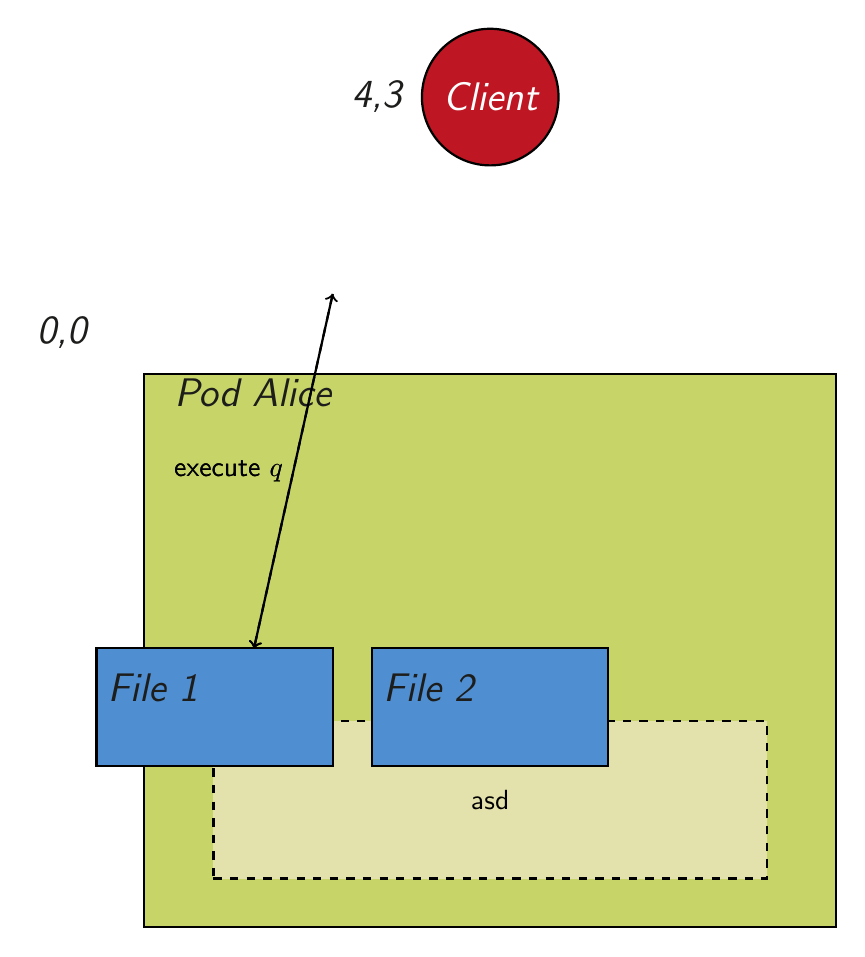
\begin{tikzpicture}[
    node distance = 20em, auto, thick,
    title/.style={text=colortext,font={\Large\itshape}},
    titlewhite/.style={text=colorwhite,font={\Large\itshape}},
    person/.style={text=colorwhite,font={\Large\bfseries}},
    code/.style={text=colortext,font={}},
    key/.style={text=colorkey,font={\tiny\itshape}}
]
\coordinate (center) at (0,0);
\coordinate (center_client) at (4,3);
\coordinate (center_client2) at (4,4);

\node[title,text width=10em] at (center) {0,0};
\node[title,text width=10em] at (center_client) {4,3};

% \path[every node/.style={font=\sffamily\small}, ->]
% 	(1) edge node [pos=0.4, fill=yellow!20] {o$_1$:hasID} (1a)
% 	(1) edge node [yshift=0.05cm,fill=yellow!20] {o$_1$:cables} (2)
% 	(2) edge node [xshift=0.5cm,fill=yellow!20] {o$_1$:bandwidth} (3)
% 	(4) edge node [xshift=0.8cm, fill=yellow!20] {} (2)
% 	(5) edge node [xshift=-0.8cm,yshift=-0.1cm, fill=yellow!20] {rdfs:subClassOf} (2);


\node[draw,fill=colorclient,circle,text centered, minimum height=1em] (rect) at (center_client)  [titlewhite,align=center, text width=4em] {Client};
\node[draw,fill=colorpod,rectangle,below of = rect, minimum height=20em, minimum width=25em] (POD) {};
\node[below right, text depth=20mm,text height=5mm,,title,text width=10em] at (POD.north west){} ++(1.75,-0.75) node[title,text width=10em] {Pod Alice};
\node[draw,dashed,fill=colorrepeat,fill opacity=0.5, text opacity=1,below=20em of rect, minimum height=2cm, minimum width=20em] (ACP) {asd};
    % Client
    % \draw[fill=colorclient] (0,3) rectangle (2,4);
    % \node[title,colorwhite,text width=10em] at (2,3.5) {Client};
    % \draw[fill=colorclient] (0.5,2) rectangle (3,3);
    % \node[title,colorwhite,text width=10em] at (2.5,2.5) {Planner};
    % \draw[fill=colorclient] (0.5,0.5) rectangle (3,1.5);
    % \node[title,colorwhite,text width=10em] at (2.5,1) {Executor};

    % Arrows to/from client
    % \draw[->,thick] (-5,2.5) -- node[midway]{query $Q$, sources $U$, keys $K$} (0.5,2.5);
    % \draw[<-,thick] (-5,1) -- node[midway]{query results} (0.5,1);

    % Pod Alice
    % \draw[fill=colorpod] (-1.5,-6) rectangle (6,0);
    % \node[title,text width=10em] at (0.5,-0.5) {Pod Alice};
    % \draw[dashed,fill=colorrepeat,fill opacity=0.5, text opacity=1] (-1.2,-5.7) rectangle (5.8,-1);
    \draw[fill=colorfile] (-1,-5.5) rectangle (2,-4);
    \node[title,text width=10em] at (0.9,-4.5) {File 1};
    \draw[fill=colorfile] (2.5,-5.5) rectangle (5.5,-4);
    \node[title,text width=10em] at (4.4,-4.5) {File 2};

    % % Pod Bob
    % \draw[fill=colorpod] (6.5,-6) rectangle (14,-2.5);
    % \node[title,text width=10em] at (8.5,-3) {Pod Bob};
    % \draw[fill=colorfile] (7,-5.5) rectangle (10,-4);
    % \node[title,text width=10em] at (8.9,-4.5) {File 1};
    % \draw[fill=colorfile] (10.5,-5.5) rectangle (13.5,-4);
    % \node[title,text width=10em] at (12.4,-4.5) {File 2};

    % % Pod Carol
    % \draw[fill=colorpod] (14.5,-6) rectangle (22,-2.5);
    % \node[title,text width=10em] at (16.5,-3) {Pod Carol};
    % \draw[fill=colorfile] (15,-5.5) rectangle (18,-4);
    % \node[title,text width=10em] at (16.9,-4.5) {File 1};
    % \draw[fill=colorfile] (18.5,-5.5) rectangle (21.5,-4);
    % \node[title,text width=10em] at (20.4,-4.5) {File 2};
    % \draw[dashed,fill=colorrepeat] (3.6,2.9) rectangle (8.9,0.25);
        % Summary
        % \draw[fill=colorsummary] (9,3) rectangle (14,-0.5);
        % \node[title,text width=20em] at (12.5, 2.5) {Aggregated Summary};
        % \draw[fill=colorsummary] (9.5,2) rectangle (10.5,0.25);
        % \node[code,text width=2em] at (10,1.2) {S1\\S2\\\ldots};
        % \draw[fill=colorsummary] (10.5,2) rectangle (11.5,0.25);
        % \node[code,text width=2em] at (11,1.2) {P1\\P2\\\ldots};
        % \draw[fill=colorsummary] (11.5,2) rectangle (12.5,0.25);
        % \node[code,text width=2em] at (12,1.2) {O1\\O2\\\ldots};
        % \draw[fill=colorsummary] (12.5,2) rectangle (13.5,0.25);
        % \node[code,text width=2em] at (13,1.2) {G1\\G2\\\ldots};


    % Arrows between executor and files
    \draw[<->,thick,dashed] (2,0.5) -- node[left]{execute $q$} (1,-4);
    \draw[->,thick] (2,0.5) -- node[left]{execute $q$} (1,-4);

    % \draw[<->,thick,dashed] (2,0.5) -- node[left]{execute $q$} (12,-4);
    % \draw[<->,thick,dashed] (2,0.5) -- node[right]{execute $q$} (16.5,-4);

\end{tikzpicture}
\end{document}
